\documentclass{article}
\usepackage{amsmath,amsthm}
\usepackage{amssymb,latexsym}
\usepackage{float}
\usepackage{fullpage}
\usepackage{times}

% graphs
\usepackage{tikz}
\usepackage[edges,linguistics]{forest}
\usetikzlibrary{automata,positioning,shadows,arrows.meta}

\tikzset{initial text={}}

% grammars
\usepackage{listings}

\lstset{
  basicstyle=\itshape,
  xleftmargin=3em,
  literate={->}{$\rightarrow$}{2}
           {epsilon}{$\epsilon$}{1}
}

\newtheorem{theorem}{Theorem}
\newtheorem{corollary}[theorem]{Corollary}
\newtheorem{question}[theorem]{Question}
\newtheorem{lemma}[theorem]{Lemma}
\newtheorem{observation}[theorem]{Observation}
\newtheorem{proposition}{Proposition}
\newtheorem{definition}[theorem]{Definition}
\newtheorem{claim}[theorem]{Claim}
\newtheorem{fact}[theorem]{Fact}
\newtheorem{assumption}[theorem]{Assumption}
\newtheorem{example}{Example}
\newtheorem{conjecture}[theorem]{Conjecture}
\newtheorem{alg}[theorem]{Algorithm}

\newcommand{\set}[1]{{\left\{#1\right\}}}    % braces for set notation
\newcommand{\ve}[1]{\mathbf{#1}}
\newcommand{\abs}[1]{\left\lvert #1 \right\rvert}
\newcommand{\poly}{\operatorname{poly}}
\newcommand{\complex}{{\mathbb C}}
\newcommand{\reals}{{\mathbb R}}
\newcommand{\ints}{{\mathbb Z}}
\newcommand{\nats}{{\mathbb N}}
\newcommand{\proj}[1]{\mbox{$|#1\rangle \!\langle #1 |$}}
\newcommand{\enc}[1]{\left<#1\right>}
\newcommand{\spa}[1]{\mathcal{#1}}
\newcommand{\ayes}{A_{\rm yes}}
\newcommand{\ano}{A_{\rm no}}

\begin{document}

\title{
    CMSC 303 Introduction to Theory of Computation, VCU\\
    Assignment: 5\\
    Name: Steven Hernandez
}

\date{}

\maketitle
\vspace{-10mm}

\begin{enumerate}
    \item % 1
        \begin{enumerate}
            \item
                Configuration of a Turing Machine consists of

                \begin{enumerate}
                    \item
                        State
                    \item
                        Head position
                    \item
                        Tape contents
                \end{enumerate}
            \item
                Yes, a turing machine can write anything that is in the tape's alphabet $\Gamma$.
            \item
                $\Gamma$ can $ = \Sigma$, however this may cause ambiguity.
                A blank space usually indicates the end of the string, but if \textvisiblespace $\in \Sigma$, there is no knowing for certain the character indicates the end of the string.
            \item
                It depends on how a turing machine is defined.
                By our definition, a step for the turing machine either moves the head left or right.
                The head cannot remain in place.

                However, a turing machine can be defined to allow a step to move the left, right or stay in place.
                This new definition of a turing machine is equal in power to the previous turing machine.
                This is because we can simply take any steps that say to stay in place and separate them into two steps:
                move left, then move right.
                This effectively keeps the head in place.
            \item
                By our definition the turing machine's set of states $Q = \set{q_{accept}, q_{reject}}$.

                It could be the case that the turing machine will never halt in one of those two states, but still the state is still present in $Q$.
            \item
                A decidable language, when put into a Turing Machine will halt in either a rejecting or accepting state after some finite number of steps.

                On the other hand, a Turing-recognizable language can either reject, accept or loop for an unknown and possibly infinite sequence.
        \end{enumerate}
    \item % 2
        $L = \set{x | x \text{ contains twice as many 0s as 1s}}$.

        $M = $ "On input string w:

        \begin{enumerate}
            \item
                Starting from the left, move towards the end of the input to ensure there are an even number of zeros, if not, reject.
            \item
                Return to the left, scan right until the first uncrossed zero. Cross it off.
            \item
                Continue right until the next zero. Cross it off as well.
            \item
                Move all the way to the right most symbol in the input.
            \item
                Scan left until a non-crossed-off one is found. If no one is found, reject.
                Otherwise, cross off the one and return the head to the left.
            \item
                Repeat the second step until no zeros are found.
            \item
                Once scanning from left to right finds no zeros, check to see if there are any uncrossed ones.
                If there are, reject. Otherwise, accept.
        \end{enumerate}
    \item % 3
        \begin{enumerate}
            \item
                First, we determine what sort of differences there are between the two models.

                \begin{enumerate}
                    \item
                        If the head of our turing machine is on the first symbol of the tape and then is instructed to move left, the head stays in place.
                        Alternatively, the doubly infinite tape will successfully move left.
                \end{enumerate}

                To simulate this feature of our standard Turing Machine, we simply add a few conditions to our new TM.
                We begin our turing machine by marking the first symbol in some unique way so as to identify it as our initial position.
                Then we add the condition that if we try to move left but we read this unique identifying mark, we instead remain in place (or move left, then automatically move right).
            \item
                Not caring about any efficiency, we again mark our first place on the tape with a unique identifier. (Note this does not remove our turing machines ability to read the symbol below the mark).
                Then, whenever we try to move left when we see this unique identifying mark, we shift all the contents of the tape over to the left once.
                After shifting, we remove the unique identifying mark and place it on the new first space on the tape (which we will assume would be filled with a blank space symbol).
            \item
                Because the models can both recreate the mechanisms of one another, this means both are able to recognize the same set of languages.
        \end{enumerate}
    \item % 4
        \begin{enumerate}
            \item
                Use the fact that when decidable languages are defined with a Turing machine, the turing machine is gauranteed to halt, either accepting or rejecting by the definition of decidablity.
                Because of this, if we have some Turing Maching $M_1$ which recognizes the decidable language $L_1$ and a second Turing Maching $M_2$ which recognizes the decidable language $L_2$, we can show that $M_1 \circ M_2$ is also decidable.
                We simply apply the same steps from both $M_1$ and $M_2$.
                We begin with the rules $M_1$ and once our Turing Machine reaches the accepting state for $M_1$, then we begin looking at the rules for $M_2$.
                From here, we follow the rules for $M_2$ until we reach the accepting state for $M_2$.
                Obviously, if we were to have reached a rejecting state in either $M_1$ or $M_2$, then we would also enter a rejecting state for this new Turing Machine as well.
            \item
                For this, we develop a new Nondeterministic Turing Machine $M_N$.
                This NTM will attempt will run through the input string $x = yz$ where $y$ is recognized by the first Turing Machine and $z$ is recognized by the second.
                Before each character is read, our NTM will create two branches of computation such that the first branch assumes that $y$ is complete and $z$ will begin immediately upon reading the next character.
                The second branch will assume that $y$ is not yet complete, and will continue reading symbols from the input and repeat the branching behaviour before the next character is read.
                Because we are checking if $y$ is recognized by the first TM and $z$ by the second for all possible compbinations of $yz$, if any of the possible branches find both $y$ and $z$ accept, then the whole machine should accept as well.
        \end{enumerate}
    \item % 5
        Understanding a 1-PDA can recognize context-free languages, and knowing $L = \set{a^nb^nc^n | n \ge 0}$. We can simply show that a 2-PDA is more powerful, because it can recognize $L$.

        Beforehand though, we can understand that a 2-PDA is at least equivelant to a 1-PDA, because while the 2-PDA has two stacks, we can leave a stack alone during some computation and we it can effectively be used as a 1-PDA.

        To show $L$ is recognized by a 2-PDA.

        We can do this with a state diagram as seen below.
        Remember, a 1-PDA's transitions are labeled $x, y \rightarrow z$ where $x$ is the symbol read from the input, $y$ is the symbol popped off the stack and $z$ is the symbol pushed onto the stack.

        For our 2-PDA, we label transitions: $x,y_1,y_2\rightarrow z_1,z_2$ where $x$ again is the symbol read from the input.
        $y_n$ is popped from stack $n$. $z_n$ is pushed onto stack $n$.

        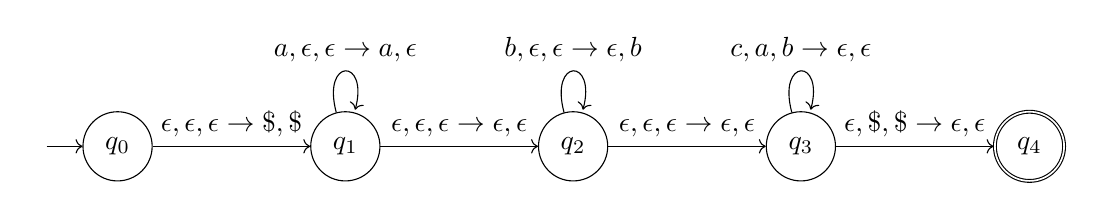
\begin{tikzpicture}
           \node[state,initial] (q_0)   {$q_0$};
           \node[state] (q_1) [right=2cm of q_0] {$q_1$};
           \node[state] (q_2) [right=2cm of q_1] {$q_2$};
           \node[state] (q_3) [right=2cm of q_2] {$q_3$};
           \node[state,accepting] (q_4) [right=2cm of q_3] {$q_4$};
            \path[->]
            (q_0) edge [above] node {$\epsilon,\epsilon,\epsilon\rightarrow\$,\$$} (q_1)
            (q_1) edge [above] node {$\epsilon, \epsilon, \epsilon \rightarrow \epsilon, \epsilon$} (q_2)
                  edge [loop above] node {$a, \epsilon, \epsilon \rightarrow a, \epsilon$} (q_1)
            (q_2) edge [above] node {$\epsilon, \epsilon, \epsilon \rightarrow \epsilon, \epsilon$} (q_3)
                  edge [loop above] node {$b, \epsilon, \epsilon \rightarrow \epsilon, b$} (q_2)
            (q_3) edge [above] node {$\epsilon, \$, \$ \rightarrow \epsilon, \epsilon$} (q_4)
                  edge [loop above] node {$c, a, b \rightarrow \epsilon, \epsilon$} (q_3)
            ;
        \end{tikzpicture}

        Thus, a 2-PDA can recognize at least on additional language, thus a 2-PDA is more powerful than a 1-PDA.
\end{enumerate}

\end{document}
